\documentclass[12pt]{amsart}
\usepackage{geometry}                % See geometry.pdf to learn the layout options. There are lots.
\geometry{letterpaper}                   % ... or a4paper or a5paper or ... 
%\geometry{landscape}                % Activate for for rotated page geometry
%\usepackage[parfill]{parskip}    % Activate to begin paragraphs with an empty line rather than an indent
\usepackage{graphicx}
\usepackage{amssymb}
\usepackage{epstopdf}
\usepackage{listings}
\usepackage{color}
\usepackage{python}
\usepackage{setspace}
 \onehalfspacing
\definecolor{codegreen}{rgb}{0,0.6,0}
\definecolor{codegray}{rgb}{0.5,0.5,0.5}
\definecolor{codepurple}{rgb}{0.58,0,0.82}
\definecolor{backcolour}{rgb}{0.95,0.95,0.92}
 
 \usepackage{xcolor}
\lstset { %
    language=C++,
    backgroundcolor=\color{black!5}, % set backgroundcolor
    basicstyle=\footnotesize,% basic font setting
}

 
\lstdefinestyle{mystyle}{
    %backgroundcolor=\color{backcolour},   
    commentstyle=\color{codegreen},
    keywordstyle=\color{magenta},
    numberstyle=\tiny\color{codegray},
    stringstyle=\color{codepurple},
    basicstyle=\footnotesize,
    breakatwhitespace=false,         
    breaklines=true,                 
    captionpos=b,                    
    keepspaces=true,                 
    numbers=left,                    
    numbersep=5pt,                  
    showspaces=false,                
    showstringspaces=false,
    showtabs=false,                  
    tabsize=2
}
 
\lstset{style=mystyle}
\DeclareGraphicsRule{.tif}{png}{.png}{`convert #1 `dirname #1`/`basename #1 .tif`.png}

\title{Finite Element Analysis for Advection Diffusion Equation}
\author{Carter Rhea}
\date{\today}                                           % Activate to display a given date or no date

\begin{document}
\maketitle


\tableofcontents

\pagebreak
\section{Abstract}
In order to better understand the Finite Element Method from a programmers point of view, this project is a tutorial in programming a robust finite element solver in python from scratch. A large component of the project is consumed with the development of Object Oriented Programming techniques allowing for a generalized solver. Moreover, this paper explores the complexities of the Advection Diffusion Equation and how it leads to the use of stability techniques in Finite Element Analysis. The primary stability technique examined in this paper is the Galerkin Lease Squares method.

\pagebreak
\section{Introduction to the Advection Diffusion Equation}
$$-k*\nabla^2u+q\cdot{} \nabla u - f  = 0 \ \ u \in \Omega$$
$$ u = 0 \ \ u \in \Gamma$$
$$k>0 \ ; \ q \ is \ a \ constant \ vector \ field$$

\subsection{Weak Formulation}
We will be following the common steps in putting the normal (strong) advection diffusion equation into its weak, or variational, form.\\
Note:$$\int_\Omega{w \nabla^2 u d\Omega}  = \int_{\delta \Gamma}{w \nabla u \cdot{} \hat{n} d\Gamma} - \int_{\Omega}{\nabla w \nabla u d\Omega}$$

Derivation:
$$\int{w(-k*\nabla^2u+q\cdot{} \nabla u - f )d\Omega} $$

$$-\int_{\delta \Gamma}{w k  \nabla u \cdot{} \hat{n} d\Gamma} + \int_{\Omega}{\nabla w k  \nabla u d\Omega} + \int_{\Omega}{w q \cdot{} \nabla u d\Omega}  - \int_{\Omega}{w f d\Omega} = 0$$

$$ \int_{\Omega}{\nabla w k  \nabla u d\Omega} + \int_{\Omega}{w q \cdot{} \nabla u d\Omega}  = \int_{\Omega}{w f d\Omega}  $$ \\

For the sake of compactness, we shall use the following two defines:
$$a(u,w) = \int_{\Omega}{\nabla w k  \nabla u d\Omega} + \int_{\Omega}{w q \cdot{} \nabla u d\Omega}  $$
$$<l,w> = \int_{\Omega}{w f d\Omega} $$
\subsection{Error Analysis}
Lets define some constants to be used in the analysis of stability: \\
$$\alpha \ - \ level \ of \ "ellipticity" \ of \ PDE  $$
$$\alpha = \frac{k}{1+C} $$
$$C \ - \ Poincar\acute{e}-Friedrich \ constant$$
$M$ is the Lipschitz continuity constant which is essentially a bounding value for the derivative of a function.
$$M = K + \sqrt{C}max|q|$$
Thus we can write the error bound as the following:
$$||u-u_h||_{1,\Omega} \leq C\frac{M}{\alpha}H^k|u|_{1,\Omega} $$

Hence, the as the ratio $\frac{max|q|}{k}$ grows, the error grows!
Thus the error is determined by the constants $q$ and $k$.  In particular, we have to look at the Peclet number \cite{peclet}:
$$P_e = \frac{k*L}{q} $$ 


We need to find a way to deal with this...

\subsection{Stability}

In order to reduce the error we need to uncouple it from constants. To do this we modify the weak form of the PDE such that we subvert the undesired error dependency on the constants whilst retaining the consistency of the solution. We will have to add terms to the variational form such that it is still a solution to the initial PDE\cite{aquino}.\\
Let $R(u_h)$ be the residual. Hence $$R(u_h) =  -\kappa \nabla^2 u + q\cdot{} \nabla u_h - f$$
Hence the general structure of our stabilized form is 
$$a(u,w)+\sum\int{P(w_h)\tau R(u_h) }d\Omega - <l,w_h>=0 $$
where $P$ is a chosen operator applied to the test function and $\tau$ is the stability parameter. \\
The many different stability methods arise from the choice of $P$. 
\subsection{Galerkin Least Squares}
We will choose the Galerkin Least Squares method to drive our choice in $P$. The main concept of this stability method is to minimize the $L^2$ norm of the residual.
Let us consider the classic example of Advection-Diffusion on a $1x1$ square. 
$$\mathcal{L}u=f$$ $$u=0 \ on \ \Gamma$$

We want to solve this in the context of an optimization (minimization to be exact) problem.\\
We define the functional$$J(v)=\int_{\Omega} R(v)^2 d\Omega$$
Let $R(v) = \mathcal{L}v-f$ be our residual.\\
If terms of $\mathfrak{L}^2$ norms we have,
$$J(v) = ||R(v)||^2_{\mathfrak{L}^2} $$
In Galerkin Least squares we have 
$$\mathcal{L}w(\mathcal{L}v-f)d\Omega=0$$
And finally to put it all together for the Galerkin Method of Finite Elements we have:  
$$a(u_h,w_h)+\sum\int_{\Omega_e}\tau\mathcal{L}w_h(\mathcal{L}u_h-f)d\Omega=<l,w_h>$$


How does this translate to the advection-diffusion equation?
$$a(u_h,w_h) + \sum_e\int_{\Omega_e}\tau(\kappa\nabla^2 w_h - q \cdot{} \nabla w_h)\cdot{}(\kappa \nabla^2 u_h - q\cdot{}\nabla u_h - f)d\Omega_e  =  <l,w_h> $$

Now we are able to go about formulating our finite element method for the stabilized weak form. As always, 
$$u_h=[N]\{d\} \ and \ w_h=[N]\{d\}$$
$$\nabla u_h=[B]\{d\} \ and \ \nabla w_h=[B]\{d\}$$
$$\nabla^2 u_h=[H]\{d\} \ and \ \nabla^2 w_h=[H]\{d\}$$

So we have the following,
$$[K] = \sum_e \int_{\Omega_e} k[B]^T[B]+[N]^Tq^T[B]d\Omega_e $$
$$[Q] = \sum_e \int_{\Omega_e} \kappa^2\tau [H]^T[H]d\Omega$$
$$[P] = \sum_e \int_{\Omega_e}  \kappa\tau[H]^Tq^T[B]		d\Omega$$
$$[S] = \sum_e \int_{\Omega_e}     \tau[B]^Tqq^T[B]   d\Omega $$
$$\{F\} = \sum_e \int_{\Omega_e}  [N]^Tf		d\Omega$$
$$\{L\} = \sum_e \int_{\Omega_e}  	\tau(\kappa[H]^T-[B]^Tq)f	d\Omega	$$

Substituting these in to the weak form we have,
$$([K]+[Q]+[P]+[P^T]+[S])\{u\} = \{F\}+\{L\} $$

Finally, we have to deal with the $\tau$ that I have up until now included in my formulas, but neglected to formally define. $\tau$ is the stability coefficient, which for our use can be considered a constant value. The following relationships demonstrate the calculation of $\tau$.
$$\tau(x,P_e) = \frac{h_e}{2*|q|}\xi(P_e)$$
$$P_e = \frac{M_i|q|h_e}{2k}$$
$$\xi(P_e) =    \left\{
\begin{array}{ll}
      P_e & 0\leq P_e \geq 1 \\
      1 & P_e>1 \\
\end{array} 
\right. 
$$

$$m_i = min\{\frac{1}{3},2C_i\}$$
$$h_e=\sqrt{2}\frac{Area}{Diagonal} $$

And for this case, we know that $m_i = \frac{1}{12}$ \cite{C}.
Hence we can calculate $\tau$. 

\section{Coding}
In order to implement the GLS method for Advection-Diffusion, I first needed to have a FE solver; I opted to use the FE solver employed in my lab: MOOSE. \\
MOOSE is a Finite element software that relies heavily on object oriented programming and is written in C++. In order to construct physical models in MOOSE, the user is required to create a class which contains a piece of the weak form. For instance, in order to properly formulate the stabilized advection-diffusion problem in MOOSE, I created a number of kernels which dealt with each piece of the weak form (I.E. I had a kernel for [K]). However, in MOOSE one is required to input the non-finite formulation (i.e. weak form). So my kernels were inputted as follows:
$$K=a(u,w)$$
$$Q = \kappa^2\tau\nabla^2w\nabla^2u$$
$$P=\kappa\tau\nabla^2wq\nabla u $$
$$N = \tau q \kappa \nabla w \nabla^2u = P^T$$
$$S = \tau \nabla w q q^T \nabla u$$
$$L = -\tau f (\kappa\nabla^2w-q\nabla u)$$
$$F = -wf$$

For the particular example, $f=0$, thus I did not include the $L$ and $F$ kernels since it would be redundant for the scope of this project. \\
The mesh for the example was created using the built-in Libmesh module in MOOSE. It was created using the following script:
\begin{lstlisting}
[Mesh]
  type = GeneratedMesh # Can generate simple lines, rectangles and rectangular prisms
  dim = 2 # Dimension of the mesh
  nx = 10 # Number of elements in the x direction
  ny = 10 # Number of elements in the y direction
  xmax = 1  #
  ymax = 1  # T
  elem_type = QUAD4
  second_order = true # biquadratic elements
[]
\end{lstlisting}

Here we ensure that we are using biquadratic elements being built upon the basic bilinear elements.

%\pagebreak

\section{Analysis}
The first major effect of using the stabilization method is the convergence of the advection-diffusion equation. With $k=0.005$, $\textbf{q}= sqrt{3}$, and $L=0.1$, the basic non-stabilized method fails to converge. In comparison, the Galerkin least squares stabilized method quickly converges to the proper approximate solution.

\subsection{Convergence}
The main convergence study for this project is the convergence of solutions for the stabilized method. The following displays the convergence of solutions through the $L^2$ norm comparing differing degrees of freedom to a DoF of $100^2$.
\begin{figure}[h!]
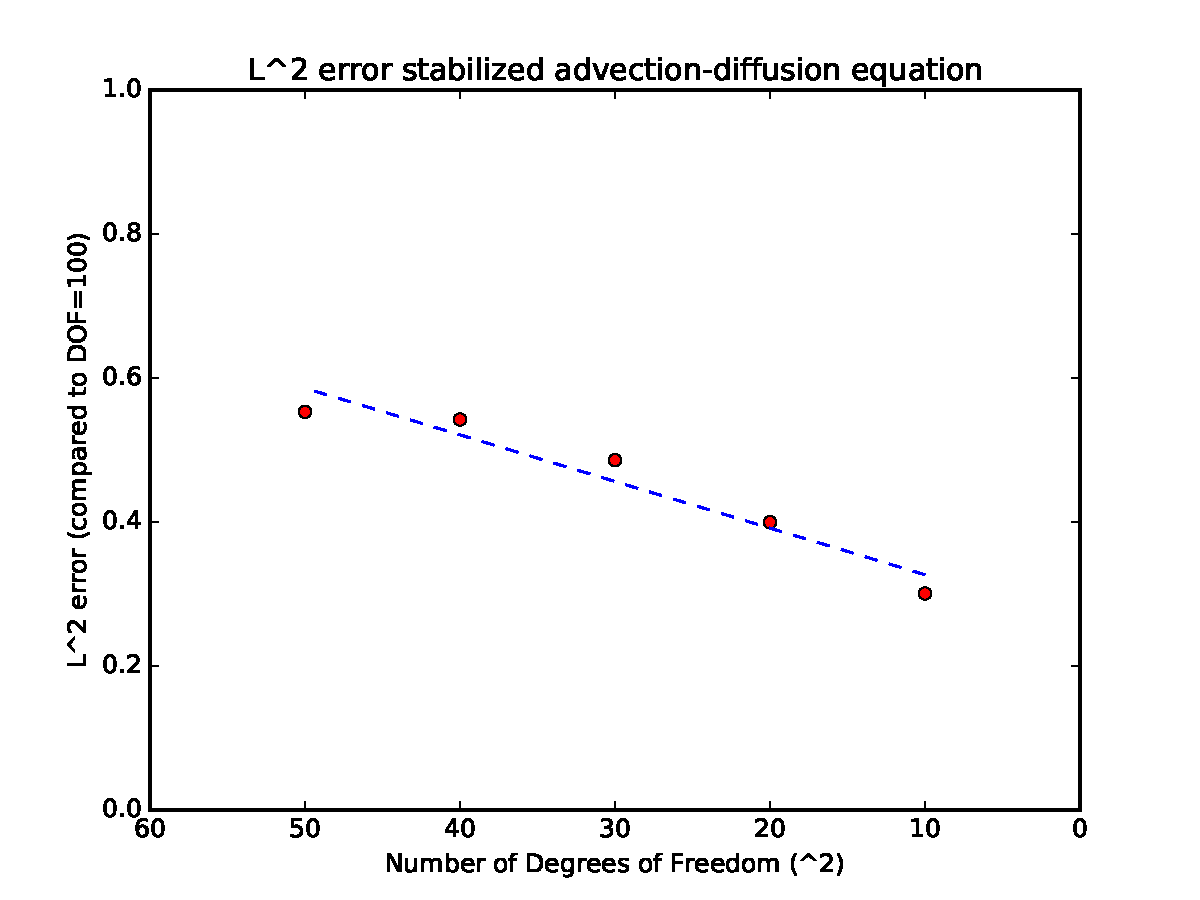
\includegraphics[width=0.8\linewidth]{L^2_error_stabilized.pdf}
\caption{Convergence of stabilized method}
\end{figure}

\begin{figure}[h!]
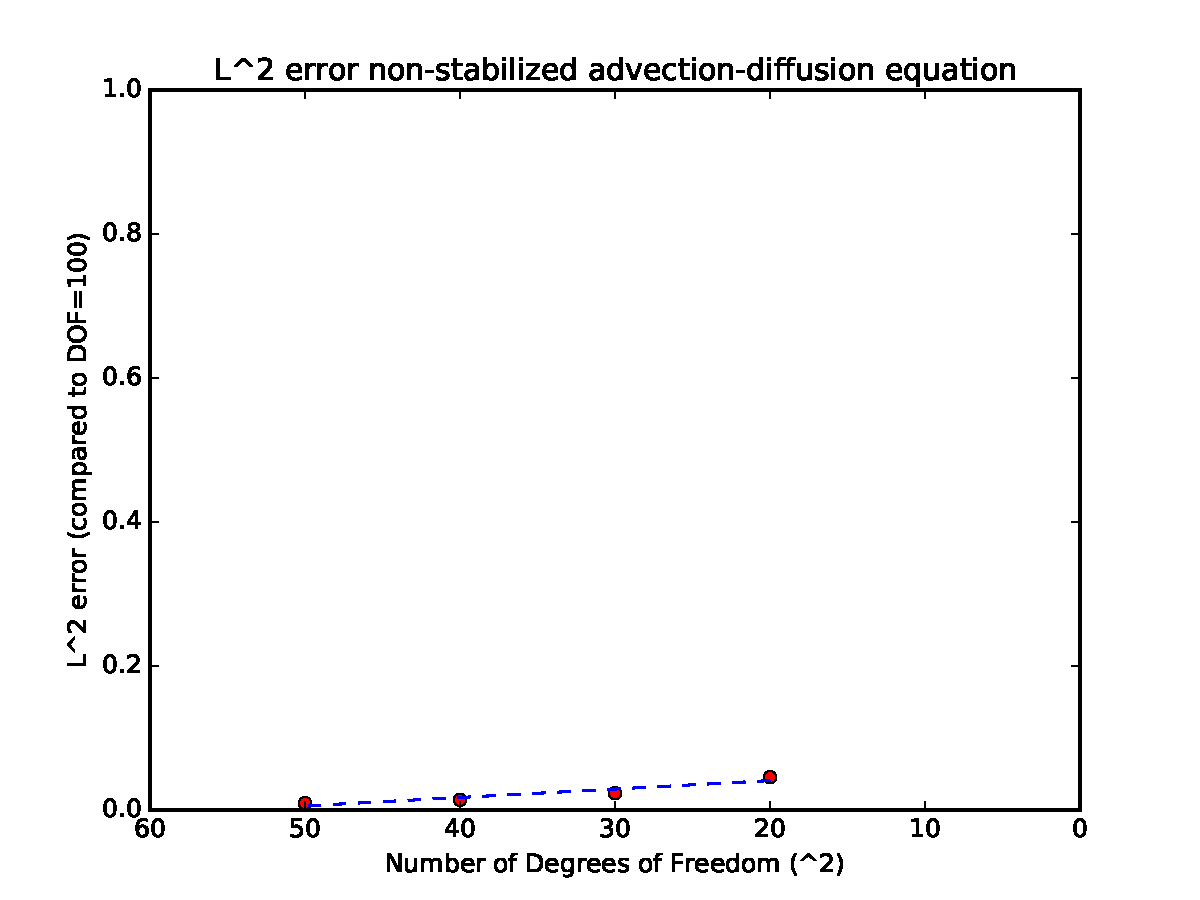
\includegraphics[width=0.8\linewidth]{L^2_error_nonstabilized.pdf}
\caption{Notice that there is no value for $DoF = 10$. This is due to the failure of convergence of the non-stablilized method for large P�clet numbers.}
\end{figure}

We can see by examining the convergence that the non-stabilized method fails to improve significantly when the mesh is refined; in comparison, the stabilized method follows an expected convergence path as the mesh is refined. The failure of convergence of the non-stabilized method is due to the large P�clet number even with a more refined mesh.





\pagebreak
\section{Appendices}
\subsection{Appendix I}
The following is a kernel in the Moose program designed to incorporate Q into the formulation.
\begin{lstlisting}
#include "Q.h"
//Q component of the stabilized GLS method for advection diffusion. See paper for details.
template<>
InputParameters validParams<Q>()
{
  InputParameters params = validParams<Kernel>();

  params.addRequiredParam<Real>("diff_constant", "this variable will be used as the diffusivity constant.");
    params.addRequiredParam<Real>("tau", "Stability parameter");
  return params;
}

Q::Q(const InputParameters & parameters) :
  Kernel(parameters),
_second_u(second()),
_second_test(secondTest()),
_second_phi(secondPhi()),
_diff_constant(getParam<Real>("diff_constant")),
_tau(getParam<Real>("tau"))

{}

Real Q::computeQpResidual()
{
    return (_diff_constant*_diff_constant)*(_tau)*_second_test[_i][_qp].tr()*(_second_u[_qp].tr()); //k^2*tau*nabla(w)*grad(u)
}

Real Q::computeQpJacobian()
{
    return (_diff_constant*_diff_constant)*(_tau)*_second_test[_i][_qp].tr()*(_second_phi[_j][_qp].tr());
}

\end{lstlisting}
\medskip

\begin{thebibliography}{9}
\bibitem{aquino}
Aquino, Wilkins. Analysis of Finite Element Methods (2016)
\bibitem{C} 
Franca et al. in their paper Stabilized FEM: I. Application to the advective-diffuse model. (CMAME 95, 1992).

\bibitem{peclet}
Patankar, Suhas V. (1980). Numerical Heat Transfer and Fluid Flow. New York: McGraw-Hill. p. 102. ISBN 0-89116-522-3.
 \end{thebibliography}

 







\end{document}  